Photomultiplier tubes are employed as photosensors in nuclear physics since decades. They detect the scintillation photons that reach its sensitive part, the photocathode, and produce an electronic signal, large enough to be easily measured. In Figure \ref{fig:SchemePMT} a schematic drawing of a PMT is given. The PMTs consists of a vacuum tube that has a glass window through which photons can penetrate. The electrons created in the photocathode travel in vacuum. The signal production has two phases:

\begin{figure}[htbp]
\centering
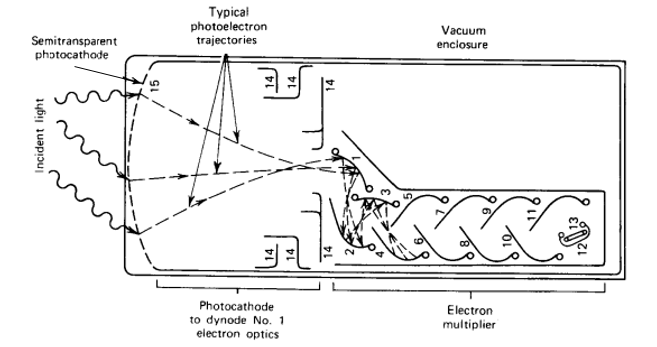
\includegraphics[scale=0.6]{3DesignPrinciples/32Tritium_detector/PMTschematic.png}
\caption{Scheme of a PMT\label{fig:SchemePMT}~\cite{Knoll}.}
\end{figure}

\begin{enumerate}
\item{} In the photocathode, photons are converted into photoelectrons through the photoelectric effect. The photocathode consists of a thin layer of material, of the order of nanometers, deposited on the inner surface of the PMT window. The material of the photocathode is chosen to optimize the probability of producing photoelectric effect with the scintillation photons. The PMTs used in different R\&D setups of the TRITIUM experiment in the University of Valencia are R8520-406 from Hamamatsu \cite{DataSheetPMTs} and the material of their photocathode is Bialkali\footnote{The bialkali material is based on the elements $\ce{^{121}_{51}Sb}$, $\ce{^{85}_{37}Rb}$ and $\ce{^{132}_{55}Cs}$}.

%The response of the PMT to long wavelengths is very small, mainly because photon energy is not enough to produce a photoelectric effect or the emitted photoelectron does not have enough energy to overcome the material work function. The response of the PMT at short wavelengths is very weak due to absorption in the window material, quartz in our case. 

The response of the PMT has a strong dependence on the energy of the photon. The quantum efficiency (QE)  spectrum, shown in Figure \ref{fig:QuantumEfficiencyPMT} for the PMTs mentioned above, is defined as the ratio of the number of photoelectrons produced at the photocathode of the PMT and the number of photons reaching it.

\begin{figure}[htbp]
\centering
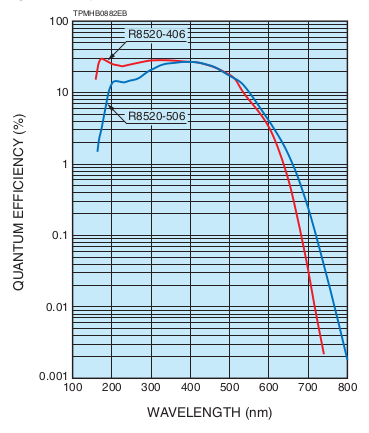
\includegraphics[scale=0.5]{3DesignPrinciples/32Tritium_detector/QuantumEfficiencyPMT.png}
\caption{Quantum efficiency spectrum for the PMT used in TRITIUM R\&D studies (R8520-406)\label{fig:QuantumEfficiencyPMT}~\cite{DataSheetPMTs}.}
\end{figure}

The maximum value of the PMT quantum efficiency is usually between $20\%$ and $30\%$ \cite{Knoll} (slightly less than $30\%$ for the PMTs used in this thesis). The emission spectrum of the scintillating fibres used, Figure \ref{fig:EmissionSpectrumFibers}, matches the quantum efficiency spectrum of the PMTs used, Figure \ref{fig:QuantumEfficiencyPMT}, and the positions of both peaks are very close, $435~\nm$ and $420~\nm$ for fibres and PMT respectively. Thus, the intrinsic efficiency of the TRITIUM detector is maximized.

\item{} As the number of photoelectrons produced in the photocatode is very small, an electron multiplication stage is employed to obtain an electronic signal of sufficient size to be processed by the electronic system. The amplification stage is based on three elements, focusing electrodes, dynodes and anode, which are metallic plates with a shape and position designed to optimize the collection and multiplication of electrons. A high voltage (HV) is applied to the PMT which is distributed between all these elements, including the photocathode, with the help of a voltage divider circuit. A positive HV, grounded in the photocathode, is convenient for measuring PMT currents, and a negative HV, grounded in the anode, gives a faster response. The electronic scheme of the voltage divider circuit of Hamamatsu is shown in Figure \ref{fig:VoltageDividerCircuit}.

\begin{figure}[h]
\centering
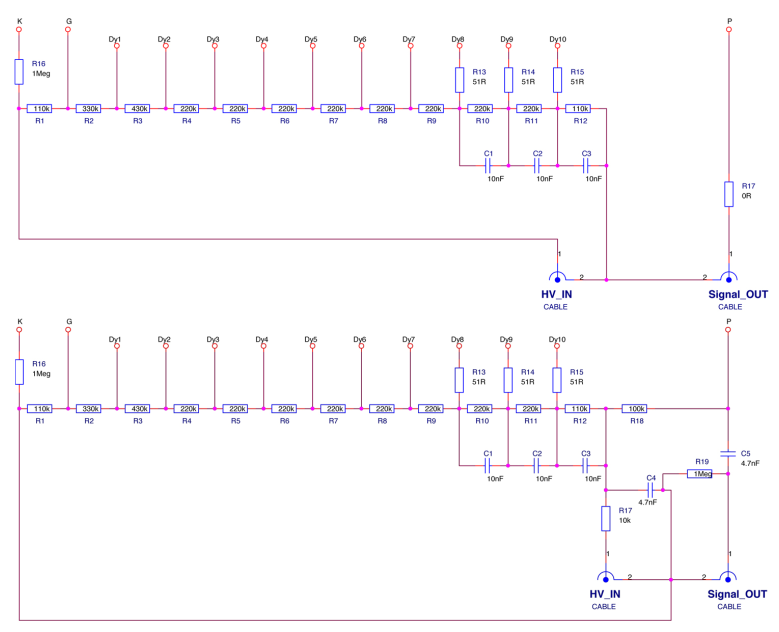
\includegraphics[scale=0.5]{3DesignPrinciples/32Tritium_detector/VoltageDividerPMT.png}
\caption{Hamamatsu commercial voltage divider electronic circuit with negative (up) and positive (below) supply high voltage\label{fig:VoltageDividerCircuit}~\cite{DataSheetPMTs}.}
\end{figure}

%The electronic circuit that can be supplied with negative voltage is faster due to the ausence of the capacitances C4 and C5, but the other circuit, supplied with positive voltage, can be interesting for other tasks like the measurement of PMT currents. We will use both, depends on the objective of the study.

Focusing electrodes guide the photoelectrons to the first dynode. They have a collection efficiency (CE) defined as the ratio of the number of photoelectrons reaching the first dynode to the number of those leaving the photocathode. The value of CE depends on the voltage between photocatode and the first dynode and reaches a $100\%$ at voltages typically above $100~\volt$. The dynodes produce the electron multiplication. A voltage difference between adjacent dynodes accelerates the electrons and produce their multiplication. The multiplication factor $\delta$ of each dynode is usually around 5 and depends on the HV. If all dynodes have the same gain, the overall gain of a PMT with N dynodes is given by \cite{Knoll},
\begin{equation}
G_{PMT} = CE\cdot{} \delta^N
\label{eq:PMTGain}
\end{equation}
and is of the order of $10^6$, strongly dependent on the applied HV.

The multiplication process follows a Poisson statistical. For each electron reaching the first dynode, $G_{PMT}$ new electrons are created with a standard deviation of $\sqrt{G_{PMT}}$. To count the number of photons that reach the PMT, the gain is eliminated and, therefore, its contribution to the counting standard deviation. This can be done by short-circuiting all the dynodes and the anode and collecting the signal directly from the first dynode. This is implemented in the voltage divider circuit used for fibre characterization, shown in Figure \ref{fig:ElectronicSchemeBasePMTNoGain}.
\begin{figure}[htbp]
\centering
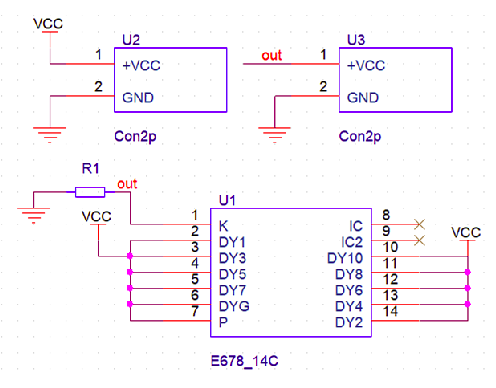
\includegraphics[scale=0.5]{3DesignPrinciples/32Tritium_detector/ElectronicSchemBasePMTNoGain.png}
\caption{Electronic scheme of the voltage divider circuit used for working with PMTs without internal gain.\label{fig:ElectronicSchemeBasePMTNoGain}}
\end{figure}
\end{enumerate}
The output pulse of a PMT has a width of the order of tens of nanoseconds and its amplitude is linear with the number of photons that reach its sensitive part up to a saturation limit, after which the linearity is lost. This limit depends on the PMT characteristics. The photocathode may emit electrons in the absence of light. Their intensity $I_{DC}$, called dark current, is due to thermoionic emission. For the PMTs employed in this work, the dark current at room temperature is around $2~\nano\ampere$ according to their data sheet.

%The characterization of the used PMTs for dark current, gain versus HV, was done at IFIC in the framework of NEXT experiment \cite{CalibrationPMTsNEXT}. 